\begin{figure*}
\centering
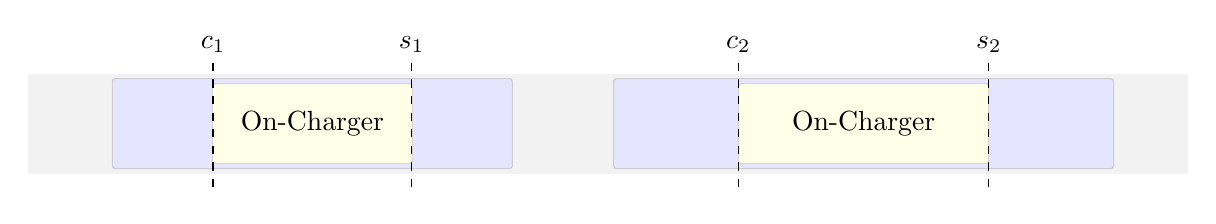
\begin{tikzpicture} 
	\node[rectangle, fill=gray!10, minimum width=5.8in, minimum height=0.5in](busSched) at (7.75,1){}; 

	\node[rectangle, draw=blue!10!black!20, fill=blue!10, minimum width=2in, minimum height=0.45in, rounded corners=1pt](busAvail1) at (4,1){In-Station};
	\node[rectangle, draw=blue!10!black!20, fill=blue!10, minimum width=2.5in, minimum height=0.45in, rounded corners=1pt](busAvail2) at (11,1){In-Station};

	\node[rectangle, draw=yellow!10!black!20, fill=yellow!10, minimum width=1in, minimum height=0.4in, rounded corners=1pt](busAvail1) at (4,1){On-Charger};
	\node[rectangle, draw=yellow!10!black!20, fill=yellow!10, minimum width=1.25in, minimum height=0.4in, rounded corners=1pt](busAvail2) at (11,1){On-Charger};


	\node(firstATop) at (2.74,2){$c_1$};
	\node(firstABtm) at (2.74,0.2){};
	\draw[dashed, line width=0.5pt](firstATop) -- (firstABtm.center);
	\node(firstDTop) at (5.26,2){$s_1$};
	\node(firstDBtm) at (5.26,0.2){};
	\draw[dashed, line width=0.5pt](firstDTop) -- (firstDBtm.center);

	\node(secondATop) at (9.41,2){$c_2$};
	\node(secondABtm) at (9.41,0.2){};
	\draw[dashed, line width=0.5pt](secondATop) -- (secondABtm.center);
	\node(secondDTop) at (12.59,2){$s_2$};
	\node(secondDBtm) at (12.59,0.2){};
	\draw[dashed, line width=0.5pt](secondDTop) -- (secondDBtm.center);


\end{tikzpicture}
\caption{Bus Charging}
\label{fig:busTime3}
\end{figure*}
